% Class Notes Template
\documentclass[12pt]{article}
\usepackage[margin=1in]{geometry} 
\usepackage[utf8]{inputenc}

% Packages
\usepackage[french, english]{babel}
\usepackage{amsmath, amsthm, amssymb ,amsfonts, graphics, tikz, float, enumerate, graphicx}
\usepackage{listings}
\usepackage{color} %red, green, blue, yellow, cyan, magenta, black, white
\definecolor{mygreen}{RGB}{28,172,0} % color values Red, Green, Blue
\definecolor{mylilas}{RGB}{170,55,241}

\lstset{language=Matlab,%
	%basicstyle=\color{red},
	breaklines=true,%
	morekeywords={matlab2tikz},
	keywordstyle=\color{blue},%
	morekeywords=[2]{1}, keywordstyle=[2]{\color{black}},
	identifierstyle=\color{black},%
	stringstyle=\color{mylilas},
	commentstyle=\color{mygreen},%
	showstringspaces=false,%without this there will be a symbol in the places where there is a space
	numbers=left,%
	numberstyle={\tiny \color{black}},% size of the numbers
	numbersep=9pt, % this defines how far the numbers are from the text
	emph=[1]{for,end,break},emphstyle=[1]\color{blue}, %some words to emphasise
	%emph=[2]{word1,word2}, emphstyle=[2]{style},    
}

% Title
\title{ECON 6140 - Problem Set \# 3}
\date{\today}
\author{Julien Manuel Neves}

% Use these for theorems, lemmas, proofs, etc.
\newtheorem{theorem}{Theorem}
\newtheorem{corollary}[theorem]{Corollary}
\newtheorem{lemma}[theorem]{Lemma}
\newtheorem{observation}[theorem]{Observation}
\newtheorem{proposition}[theorem]{Proposition}
\newtheorem{definition}[theorem]{Definition}
\newtheorem{claim}[theorem]{Claim}
\newtheorem{fact}[theorem]{Fact}
\newtheorem{assumption}[theorem]{Assumption}
\newtheorem{problem}[theorem]{Problem}
\newtheorem{set-up}[theorem]{Set-up}
\newtheorem{example}[theorem]{Example}
\newtheorem{remark}[theorem]{Remark}
\newtheorem{axiom}[theorem]{Axiom}

% Usefuls Macros
\newcommand{\field}[1]{\mathbb{#1}}
\newcommand{\N}{\field{N}} % natural numbers
\newcommand{\R}{\field{R}} % real numbers
\newcommand{\Z}{\field{Z}} % integers
\newcommand\F{\mathcal{F}}
\newcommand\B{\mathbb{B}}
\renewcommand{\Re}{\R} % reals
\newcommand{\Rn}[1]{\mathbb{R}^{#1}}
\newcommand{\1}{{\bf 1}} % vector of all 1's
\newcommand{\I}[1]{\mathbb{I}_{\left\{#1\right\}}} % indicator function
\newcommand{\La}{\mathscr{L}}
% \newcommand{\tends}{{\rightarrow}} % arrow for limits
% \newcommand{\ra}{{\rightarrow}} % abbreviation for right arrow
% \newcommand{\subjectto}{\mbox{\rm subject to}} % subject to

%% math operators
\DeclareMathOperator*{\argmin}{arg\,min}
\DeclareMathOperator*{\argmax}{arg\,max}
\DeclareMathOperator*{\maximize}{maximize}
\DeclareMathOperator*{\minimize}{minimize}
\DeclareMathOperator{\E}{\mathsf{E}} % expectation
\newcommand{\Ex}[1]{\E\left\{#1\right\}} % expectation with brackets
\DeclareMathOperator{\pr}{\mathsf{P}} % probability
\newcommand{\prob}[1]{\pr\left\{#1\right\}}
\DeclareMathOperator{\subjectto}{{s.t.\ }} % subject to
\newcommand{\norm}[1]{\left\|#1\right\|}
\newcommand{\card}[1]{\left|#1\right|}

% Extra stuff
\newcommand\seq[1]{\{ #1 \}}
\newcommand{\inp}[2]{\langle #1, #2 \rangle}

\newcommand{\inv}{^{-1}}

\newcommand{\pa}[1]{\left(#1\right)}
\newcommand{\bra}[1]{\left[#1\right]}
\newcommand{\cbra}[1]{\left\{ #1 \right\}}

\newcommand{\pfrac}[2]{\pa{\frac{#1}{#2}}}
\newcommand{\bfrac}[2]{\bra{\frac{#1}{#2}}}

\newcommand{\mat}[1]{\begin{matrix}#1\end{matrix}}
\newcommand{\pmat}[1]{\pa{\mat{#1}}}
\newcommand{\bmat}[1]{\bra{\mat{#1}}}

\begin{document}

\maketitle

\section*{Open Sector Growth Model via Dynamic Programming}

\begin{enumerate}[(1)]
	\item 
	Let $\tau_t^c=\tau^c$ and $\tau_t^x=\tau^x$ be constant. The functional equation is given by	
	\[
	(Tv)(k)=\max_{0\leq k' \leq \frac{f(k)}{(1+\tau^x)}+ (1-\delta)k} \left\lbrace u\left( \frac{f(k)}{(1+\tau^c)}- \frac{(1+\tau^x)}{(1+\tau^c)}(k'-(1-\delta)k) \right)  +\beta v(k')\right\rbrace 
	\]
	\item 
	Our state variable is the current value of $k$ and our control is the future value of capital $k'$. 
	
	In our setting, this makes sense since we can't affect the current value of capital, but we can decide how much to consumes/invest to pinpoint capital in the next period.
	
	Note that we can't set our state space equal to $[0,1]$. In fact, part 4-7 shows a steady state value of capital that is not even remotely close to be inside $[0,1]$.
	
	\item 
	
	Note that $T$ is defined on a the set of bounded function defined on $[0.\infty)$.
	
	To show that $T$ is a contraction, we can use Blackwell's theorem. In fact, we only need to show monotonicity and discounting for $T$
	\begin{enumerate}[(i)]
		\item Monotonicity
		
		Let $v(x)\leq w(x)$ and $g_v(k)$, $g_w(k)$ be the respective policy function. Then,
		\begin{align*}
			(Tv)(k)&=\max_{0\leq k' \leq \frac{f(k)}{(1+\tau^x)}+ (1-\delta)k} \left\lbrace u\left( \frac{f(k)}{(1+\tau^c)}- \frac{(1+\tau^x)}{(1+\tau^c)}(k'-(1-\delta)k) \right)  +\beta v(k')\right\rbrace \\
			& =u\left( \frac{f(k)}{(1+\tau^c)}- \frac{(1+\tau^x)}{(1+\tau^c)}(g_v(k)-(1-\delta)k) \right)  +\beta v(g_v(k)) \\
			& \leq u\left( \frac{f(k)}{(1+\tau^c)}- \frac{(1+\tau^x)}{(1+\tau^c)}(g_v(k)-(1-\delta)k) \right)  +\beta w(g_v(k)) \\
			& \leq u\left( \frac{f(k)}{(1+\tau^c)}- \frac{(1+\tau^x)}{(1+\tau^c)}(g_f(k)-(1-\delta)k) \right)  +\beta w(g_w(k)) \\
			&=\max_{0\leq k' \leq \frac{f(k)}{(1+\tau^x)}+ (1-\delta)k} \left\lbrace u\left( \frac{f(k)}{(1+\tau^c)}- \frac{(1+\tau^x)}{(1+\tau^c)}(k'-(1-\delta)k) \right)  +\beta w(k')\right\rbrace \\
		\Rightarrow	(Tv)(k)& \leq (Tw)(k)
		\end{align*}
		\item Discounting
			\begin{align*}
		(Tv+a)(k)&=\max_{0\leq k' \leq \frac{f(k)}{(1+\tau^x)}+ (1-\delta)k} \left\lbrace u\left( \frac{f(k)}{(1+\tau^c)}- \frac{(1+\tau^x)}{(1+\tau^c)}(k'-(1-\delta)k) \right)  +\beta (v(k')+a)\right\rbrace \\
		&=\max_{0\leq k' \leq \frac{f(k)}{(1+\tau^x)}+ (1-\delta)k} \left\lbrace u\left( \frac{f(k)}{(1+\tau^c)}- \frac{(1+\tau^x)}{(1+\tau^c)}(k'-(1-\delta)k) \right)  +\beta v(k')\right\rbrace +\beta a \\
		&= (Tv)(k) +\beta a
		\end{align*}
	\end{enumerate}

Hence, $T$ is a contraction.
	\item
	
Figure \ref{fig:fig1} show the value function around the steady state and Figure \ref{fig:fig2} shows the policy function.
	\begin{figure}[H]
		\centering
		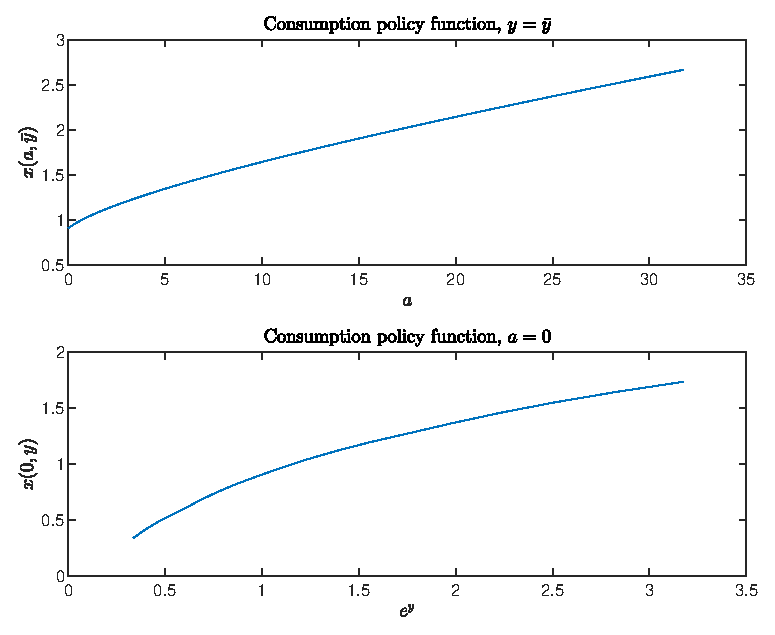
\includegraphics[width=0.7\linewidth]{fig1}
		\caption{Value function}
		\label{fig:fig1}
	\end{figure}
	\begin{figure}[H]
		\centering
		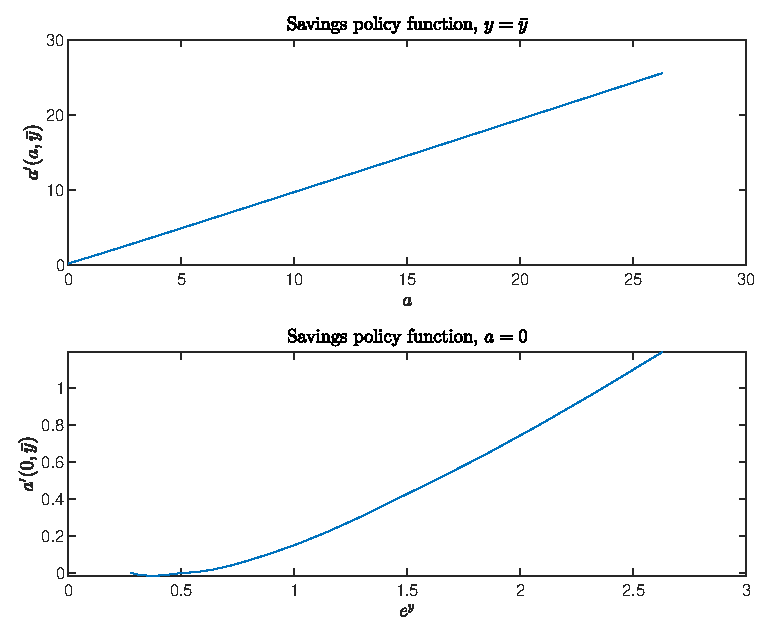
\includegraphics[width=0.7\linewidth]{fig2}
		\caption{Policy function}
		\label{fig:fig2}
	\end{figure}

	\item
	
Figure \ref{fig:fig3} show the time path of capital starting from $k_0=0.9k^*$.
	\begin{figure}[H]
		\centering
		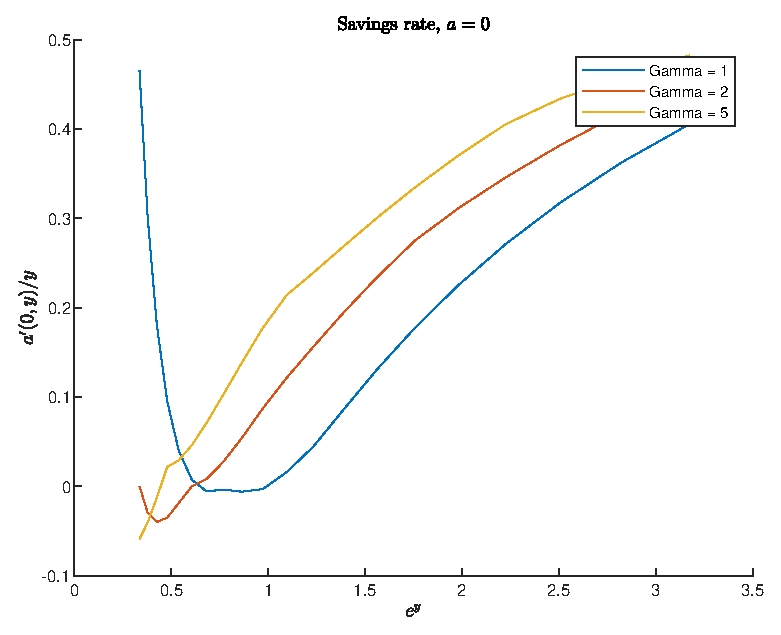
\includegraphics[width=0.7\linewidth]{fig3}
		\caption{Time path for consumption and capital}
		\label{fig:fig3}
	\end{figure}

	\item
	
	We use the shooting algorithm for this question. For sake of clarity, we provide the dynamic equations:
	\begin{align*}
		k_{t+1} &= \frac{k_t^\alpha}{(1+\tau^x_t)}+(1-\delta)k_t-c_t\frac{(1+\tau^c_t)}{(1+\tau^x_t)}\\
		c_{t+1} &= c_t\left( \frac{(1+\tau^c_t)(1+\tau^x_{t+1})}{(1+\tau^x_t)(1+\tau^c_{t+1}))}\right)^\frac{1}{\sigma}\left( \frac{\alpha\beta k_t^{\alpha-1}}{(1+\tau^x_{t+1})}+\beta(1-\delta))\right) ^\frac{1}{\sigma}
	\end{align*}
	
	
	Figure \ref{fig:fig4} show the time path of capital for a permanent tax increase. Note that the consumption jumps at $t=1$ to get back to the steady path.
	\begin{figure}[H]
		\centering
		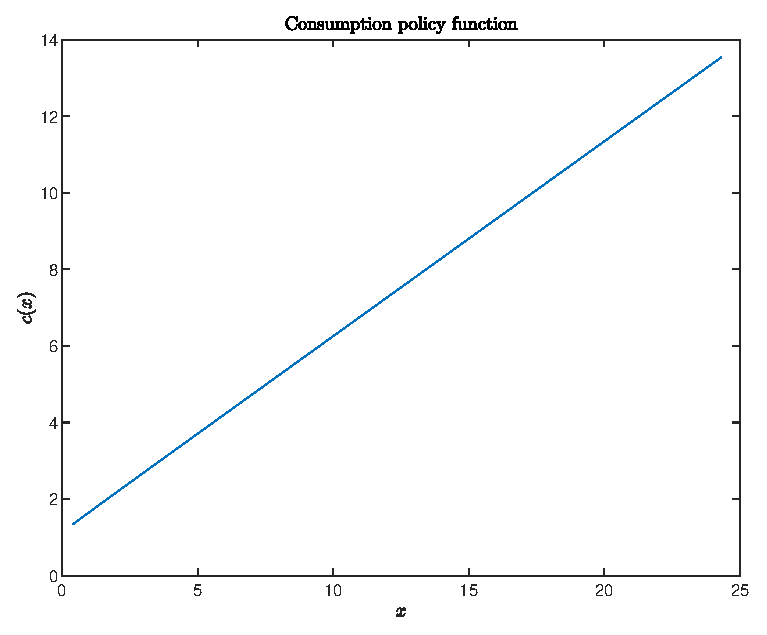
\includegraphics[width=0.7\linewidth]{fig4}
		\caption{Time path for consumption and capital}
		\label{fig:fig4}
	\end{figure}

	\item
	
	Again we use the shooting algorithm for this question. Figure \ref{fig:fig5} show the time path of capital for a temporary tax increase. 
	
	In this setting, the steady path moves both at $t=1$ and $t=10$ explaining the two jumps in consumption to insure that we will reach the steady state in the future. 
	\begin{figure}[H]
		\centering
		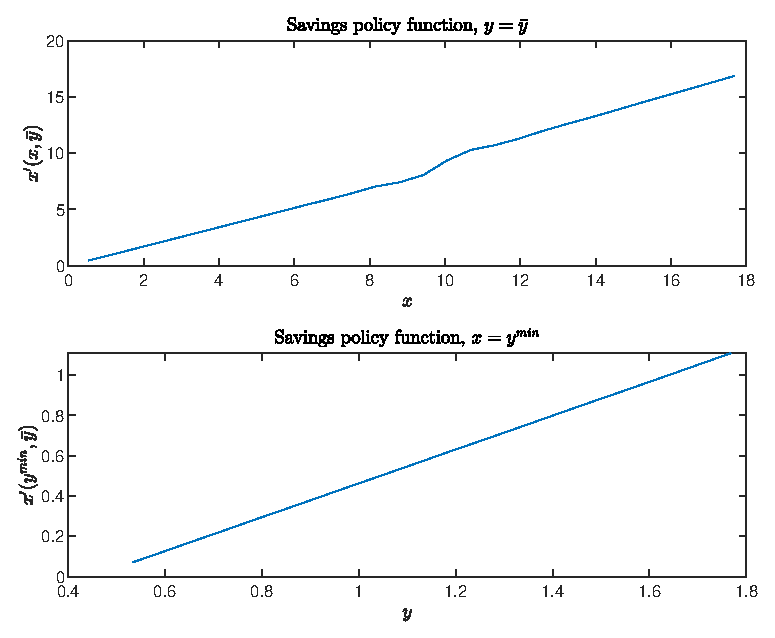
\includegraphics[width=0.7\linewidth]{fig5}
		\caption{Time path for consumption and capital}
		\label{fig:fig5}
	\end{figure}


\end{enumerate}

\section*{Ben-Porath}
\begin{enumerate}[(1)]
	\item 
	
	\begin{enumerate}[(i)]
		\item $\Rightarrow$
		
		Let $Y^*=\max_{s(t),h(t)}\int_{0}^{\infty}\exp(-rt)w(t)(1-s(t))h(t)dt$ and $\cbra{c(t),s(t),h(t)}_{t=0}^\infty$ solve the household problem.
		
		Let's assume that $\cbra{s(t),h(t)}$ does not maximizes $\int_{0}^{\infty}\exp(-rt)w(t)(1-s(t))h(t)dt$, i.e. $\exists Y$ such that
		\[
		\int_{0}^{\infty}\exp(-rt)w(t)(1-s(t))h(t)dt = Y < Y^*
		\]
		
		Let $c'(t)=c(t)+\epsilon$ for some $\epsilon>0$. Clearly, $c' \succ c$ due to strictly increasing nature of $u(\cdot)$. If, we can find an $\epsilon$ such that $c'(t)$ is feasible, then we have a contradiction with $\cbra{c(t),s(t),h(t)}_{t=0}^\infty$ solving the household problem.
		
		\begin{align*}
			\int_{0}^{\infty}\exp(-rt)c'(t)dt & = \int_{0}^{\infty}\exp(-rt)c(t)dt + \int_{0}^{\infty}\exp(-rt)\epsilon dt\\
			& \leq \int_{0}^{\infty}\exp(-rt)w(t)(1-s(t))h(t)dt + \frac{\epsilon}{r}\\
			& \leq Y + \frac{\epsilon}{r}
		\end{align*}
		
		Since $Y<Y'$, there exists an $\epsilon>0$ such that $Y + \frac{\epsilon}{r}\leq Y^*$. Hence, there exists some $\cbra{s'(t),h'(t)}_{t=0}^\infty$ such that $\int_{0}^{\infty}\exp(-rt)w(t)(1-s'(t))h'(t)dt=Y^*$ which implies that $\cbra{c'(t),s'(t),h'(t)}_{t=0}^\infty$ is feasible, i.e. we have a contradiction.
		
		\item $\Leftarrow$
		
		Let $\cbra{s(t),h(t)}_{t=0}^\infty$ solve $\max_{s(t),h(t)}\int_{0}^{\infty}\exp(-rt)w(t)(1-s(t))h(t)dt = Y$.
		
		Let $\cbra{c(t)}_{t=0}^\infty$ solve the household problem and $\cbra{c'(t)}_{t=0}^\infty$ be any solution such that $c'\succ c$. 
		
		Since $\cbra{c(t)}_{t=0}^\infty$ solves the household problem with the following budget constraint,
		\[
		\int_{0}^{\infty}\exp(-rt)c(t)dt \leq Y
		\]
		we have that 
		\[
		\int_{0}^{\infty}\exp(-rt)c'(t)dt > Y
		\]
		
		Therefore, any $\cbra{s'(t),h'(t)}_{t=0}^\infty$ that supports $\cbra{c'(t)}_{t=0}^\infty$ it must be the case that $int_{0}^{\infty}\exp(-rt)w(t)(1-s'(t))h'(t)dt>Y$ which is a contradiction. 
		
		Hence, $\cbra{c(t),s(t),h(t)}_{t=0}^\infty$ solves the household problem.
		
	\end{enumerate}
	\item 
	The current Hamiltonian is given by
	\[
	\mathcal{H}(s,h,\mu) = w(t)(1-s(t))h(t)+\mu(t)(\phi(s(t)h(t))-\delta_hh(t))
	\]
	where $h$ is the state variable, $s$ the control variable and $\mu$ the costate variable.
	
	The FOCs, TVC, and constraint are given by
	\begin{align*}
		s&: -w(t)h(t)+\mu(t)h(t)\phi'(s(t)h(t)) = 0\\
		h&: w(t)(1-s(t))+\mu(t)(s(t)\phi'(s(t)h(t))-\delta_h)  = r\mu(t)-\dot{\mu}(t)\\
		TVC&: \lim_{t\to \infty} \exp(-rt)\mu(t)h(t)=0\\
		&: \dot{h} = \phi(s(t)h(t))-\delta_hh(t)
	\end{align*}
	
	
	\item 
	
	First, we differentiate the first FOC
	\[
	{\mu}(t)\phi''(x(t))\dot{x}(t)+\phi'(x(t))\dot{\mu}(t)= \dot{w}(t) 
	\]
	
	We can then combine the FOCs in the following way
	\begin{align*}
	-\dot{\mu}(t) &=w(t)(1-s(t))+\frac{w(t)}{\phi'(x(t))}(s(t)\phi'(x(t))-\delta_h-r)  \\
	-\dot{\mu}(t) &= w(t)+\frac{w(t)}{\phi'(x(t))}(-\delta_h-r)  \\
	-\phi'(x(t))\dot{\mu}(t) &=\phi'(x(t))w(t)+w(t)(-\delta_h-r) \\
		{\mu}(t)\phi''(x(t))\dot{x}(t)-\dot{w}(t) &=\phi'(x(t))w(t)-w(t)(\delta_h+r)  \\
		\Rightarrow  \dot{x}(t) & =\frac{1}{{\mu}(t)\phi''(x(t))} (\dot{w}(t)+w(t)(\phi'(x(t))-\delta_h-r)) 
\end{align*}

\item

In steady state, $\dot{\mu}=\dot{h}=0$. Hence,
\begin{align*}
0 &= \phi(x^*(t))-\delta_hh^*(t)\\
\Rightarrow h^*(t) & = \frac{\phi(x^*(t))}{\delta_h}
\end{align*}
and
\begin{align*}
	\phi'(x^*(t))  & = \delta_h+r\\
	\Rightarrow x^*(t)  & = \phi^{'-1}(\delta_h+r)
\end{align*}

This implies that
\begin{align*}
	\Rightarrow h^*(t) &  = \frac{\phi(\phi^{'-1}(\delta_h+r))}{\delta_h}\\
\Rightarrow  s^*(t) & =  \frac{x^*(t)}{ h^*(t)} = \frac{\delta_h\phi^{'-1}(\delta_h+r)}{\phi(\phi^{'-1}(\delta_h+r))}
\end{align*}

We have that $h^*$ and $s^*$ are uniquely determined by $\delta_h$, $r$ and the shape of $\phi(\cdot)$. Note that $\phi(\cdot)$ is strictly increasing while $\phi^{'-1}(\cdot)$ is strictly decreasing. 

Additionally, $w(t)$ does not influence the steady state human capital accumulation and the schooling decision. This contrasts the fact that $w(t)$ does influence the path of $x(t)$, but not the steady state.

\end{enumerate}
	
	
\section*{Code}

\lstinputlisting[language=Matlab]{"neves_econ_6140_ps4.m"}

\end{document}
